\documentclass[sigconf,authordraft]{acmart}

%% Rights management information.
\setcopyright{acmlicensed}
\copyrightyear{2026}
\acmYear{2026}
\acmDOI{XXXXXXX.XXXXXXX}
\acmConference[SIGIR '26]{Proceedings of the 49th International ACM SIGIR Conference on Research and Development in Information Retrieval}{July 20--24, 2026}{Melbourne, Australia}
\acmISBN{978-1-4503-XXXX-X/26/07}

% Disable standard ACM reference format box to avoid errors 
% when not using a formal ACM bibliography style/database.
\settopmatter{printacmref=false}

\begin{document}

\title{Beyond the Vector Black Box: Toward Interpretable Semantic Resonance in Neural Information Retrieval}

% Yahan authors ke naam aur details add kiye gaye hain
\author{Vinay Venkatesh}
\email{vinvin@google.com}
\affiliation{%
  \institution{Google}
  \country{USA}
}

\author{Debanshu Das}
\email{debanshu@google.com}
\affiliation{%
  \institution{Google}
  \country{USA}
}

\author{Surbhi Motghare}
\email{smotghare@salesforce.com}
\affiliation{%
  \institution{Salesforce}
  \country{USA}
}

\renewcommand{\shortauthors}{Venkatesh, Das, and Motghare}

\begin{abstract}
Dense retrieval models based on Large Language Model (LLM) embeddings deliver strong semantic matching performance but introduce operational challenges in production search systems, including limited diagnostic traceability and absence of deterministic control. When retrieval errors occur, maintainers often lack mechanisms to isolate and adjust specific semantic drivers without retraining the model.

We present Interpretable Semantic Resonance (ISR), a lightweight sparse bottleneck framework that decomposes dense embeddings into steerable semantic facets while preserving retrieval topology. ISR is trained using a reconstruction, sparsity, and inner-product preservation objective and supports query-time semantic weighting via a modifier vector.

Across five BEIR subsets, ISR maintains statistically comparable NDCG@10 to its dense baseline while improving diagnostic traceability by 2–5× and enabling controlled ranking adjustments with bounded latency overhead (~9ms on NVIDIA T4). We analyze hardware, sparsity, and storage trade-offs and discuss deployment guardrails. ISR demonstrates that controllable and auditable neural retrieval can be integrated into existing dense pipelines without retraining encoders or sacrificing ANN compatibility.
\end{abstract}

%% The code below is generated by the tool at http://dl.acm.org/ccs.cfm.
\begin{CCSXML}
<ccs2012>
   <concept>
       <concept_id>10002951.10003317.10003338</concept_id>
       <concept_desc>Information systems~Retrieval models and ranking</concept_desc>
       <concept_significance>500</concept_significance>
   </concept>
   <concept>
       <concept_id>10002951.10003317.10003359.10003362</concept_id>
       <concept_desc>Information systems~Retrieval effectiveness</concept_desc>
       <concept_significance>500</concept_significance>
   </concept>
 </ccs2012>
\end{CCSXML}

\ccsdesc[500]{Information systems~Retrieval models and ranking}
\ccsdesc[500]{Information systems~Retrieval effectiveness}

\keywords{Neural Information Retrieval, Dense Retrieval, Semantic Resonance, Interpretability Gap, User Controllability, Sparse Autoencoders, Mechanistic Interpretability}

\maketitle

\section{Introduction}
The transition from exact lexical matching to neural dense retrieval represents the most significant architectural shift in Information Retrieval (IR) over the last decade. Historically, frameworks like BM25 \cite{robertson2009} provided transparent, easily debuggable scoring mechanisms based on term frequency and inverse document frequency. However, the advent of Dense Passage Retrieval (DPR) \cite{karpukhin2020} and the scaling of LLMs \cite{bendersky2023} as zero-shot embedders redefined the paradigm. Today, state-of-the-art retrieval relies on projecting queries and documents into high-dimensional latent spaces, computing relevance via vector similarity functions like Maximum Inner Product Search (MIPS) \cite{shrivastava2014}.

While these models successfully overcome vocabulary mismatch, they introduce a total loss of explainability. When a dense retriever returns an irrelevant document, engineers cannot easily trace the failure to a specific token or concept. We argue that optimizing exclusively for offline ranking metrics on leaderboards like MTEB \cite{muennighoff2023} ignores practical engineering realities. In enterprise and medical search domains, hallucinated relevance or unexplainable rankings create a severe trust deficit. We propose a shift toward Interpretable Semantic Resonance (ISR), advocating for architectures that explicitly decompose latent signals into human-navigable, behaviorally aligned semantic facets. By forcing dense representations through a sparse, interpretable bottleneck, we return agency to both the system engineer and the end user.

\section{Related Work}
Classical IR models (e.g., TF-IDF \cite{croft2010}, BM25 \cite{robertson2009}) provide exact-match tracing but suffer from vocabulary mismatch. Neural approaches like DPR \cite{karpukhin2020} and ColBERT \cite{khattab2020} solve this via continuous representations, yet they entangle semantic concepts, destroying feature-level transparency. To regain this, recent breakthroughs utilize Sparse Autoencoders (SAEs) \cite{bricken2023, cunningham2024} to disentangle polysemantic LLM neurons into monosemantic features.

Concurrently, sparse models (SPLADE \cite{formal2021}, COIL \cite{lin2021_notes}, DeepImpact/uniCOIL \cite{lin_ma2021}, SNRM \cite{zamani2017}) demonstrate that inverted indexes efficiently capture semantic weightings. For interpretability, Concept Bottleneck Models and TCAV \cite{kim2018} align representations with human-defined concepts. Crucially, ISR synthesizes these architectures with Visual Analytics (VA) principles—such as semantic interaction and exemplar-based steering (Endert et al. \cite{endert2018})—by introducing a query-side UI modifier for real-time operator debuggability.

\section{The Debugging Crisis in Neural IR}
In traditional IR, an engineer can explicitly apply negative weighting to erroneous terms; in neural retrievers, no such deterministic knobs exist. LLM embeddings rely heavily on distributional semantics, often mapping documents to similar regions based on stylistic similarities rather than strict factual relevance. When a model retrieves a document from one of these semantic clumps, maintainers are forced to blindly fine-tune the model with hard negatives. This reactive patching is computationally expensive and risks catastrophic forgetting. Evaluating retrieval using metrics like NDCG@10 fails to capture operational reality; a user presented with ten semantically close but contextually incorrect results has no agency to steer the system. This lack of controllability transforms search into a rigid oracle query rather than an interactive dialogue.

\section{The Interpretable Semantic Resonance (ISR) Framework}
To resolve this debugging crisis, we propose the Interpretable Semantic Resonance (ISR) framework, transitioning embeddings from a continuous black box into a steerable interface. As illustrated in Figure \ref{fig:isr}, the architecture acts as a transparent bridge between the dense encoder and the final retrieval ranking.

\begin{figure}[htbp]
  \centering
  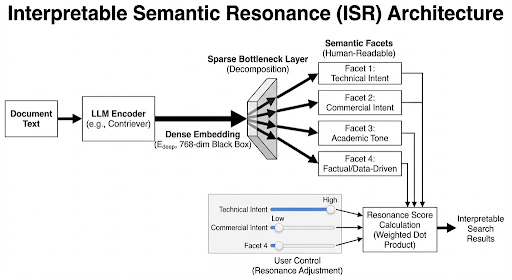
\includegraphics[width=0.9\linewidth]{fig1.png}
  \caption{The Interpretable Semantic Resonance (ISR) Architecture. Document text is processed by a standard LLM encoder into an entangled dense embedding ($E_{deep}$). The ISR Sparse Bottleneck Layer decomposes this black box into isolated, human-readable Semantic Facets. During retrieval, users adjust these facets via UI sliders (User Control), dynamically scaling the Resonance Score Calculation to produce interpretable search results.}
  \label{fig:isr}
\end{figure}

\subsection{Core Novelty and Contributions}
Standard neural IR relies on static MIPS over dense vectors. ISR introduces three primary novelties:
\begin{itemize}
    \item \textbf{Active Mechanistic Interpretability:} We transpose Sparse Autoencoders (SAEs) from an offline diagnostic tool into an active retrieval bottleneck.
    \item \textbf{Real-Time Latent Steerability:} We introduce a dynamic Resonance Loop via query-side scaling, modifying the active latent space in real-time.
    \item \textbf{The Modifier Vector ($M$):} We formalize semantic control, allowing users to explicitly up-weight or down-weight discrete latent facets via UI sliders.
\end{itemize}

\subsection{Decomposition via Sparse Bottleneck}
A document is first fed into an off-the-shelf LLM encoder (e.g., Contriever), which outputs a dense embedding $E_{deep} \in \mathbb{R}^d$ (where $d=768$). The ISR framework routes it through a Sparse Bottleneck Layer to produce a sparse feature activation vector $F$:

\begin{equation}
F = \text{ReLU}(W_{enc}E_{deep} + b_{enc})
\end{equation}

Here, $W_{enc}$ projects the dense vector into an overcomplete $k$-dimensional space (where $k \gg d$, typically $k=4096$). Because relying on an $L_1$ penalty alone is often insufficient to guarantee robust monosemanticity and can degrade ranking, we incorporate a retrieval-preserving contrastive alignment objective during dictionary learning.

\subsection{The Facet Dictionary and Resonance Score}
Because each active dimension in $F$ represents an isolated concept, we use a secondary instruction-tuned LLM to generate human-readable Semantic Facets (e.g., Facet 1: Technical Intent). During retrieval, users adjust these facets via UI sliders, generating a dynamic Modifier Vector, $M \in \mathbb{R}^k$. The final Resonance Score Calculation is computed as a weighted dot product:

\begin{equation}
S(q,d) = (F_q \odot M) \cdot F_d
\end{equation}

Because the Hadamard Product $(F_q \odot M)$ acts purely as a pre-scaling of the query vector's sparse activations, it is mathematically equivalent to a weighted dot product. $M$ can be folded entirely into the query vector at inference time, allowing compatibility with standard Approximate Nearest Neighbor (ANN) search libraries \cite{johnson2019}.

\section{Experimental Setup}
The code and resources to reproduce our experiments are publicly available at \url{https://github.com/debanshd/IR-Interpretability/tree/main}.

\subsection{Datasets, Baselines, and Hardware Requirements}
We evaluate ISR across five BEIR subsets \cite{thakur2021} (SciDocs, ArguAna, NFCorpus, FIQA, TREC-COVID) against Contriever (Dense), ColBERTv2.0 \cite{khattab2020} (Late-Interaction), and SPLADE \cite{formal2021} (Sparse Lexical).

\textbf{Baseline Selection Rationale:} While models such as E5, GTR \cite{wang2022}, and advanced Contriever variants continuously push the state-of-the-art, we selected the base Contriever, SPLADE, and ColBERTv2.0 to serve as foundational architectural representatives of the dense, sparse, and late-interaction paradigms.

\textbf{Evaluation Constraints and Subset Variance:} To ensure computational feasibility on a single NVIDIA T4 GPU, experiments were conducted using subset-sampled evaluations. Because this evaluation isolates structural tradeoffs, certain absolute baseline metrics inherently diverge from standard BEIR leaderboards. Evaluating on a constrained document pool artificially inflates absolute NDCG scores on datasets like TREC-COVID. However, because our central claim relies on the relative delta between the Contriever baseline and the ISR projection within the exact same subset, the absolute inflation does not invalidate paired statistical comparisons.

\subsection{The Composite Loss Function}
The ISR bottleneck is trained directly on the target corpus embeddings using a batch size of 64 for 150 epochs. The similarity matrices for the Inner Product Preservation (IP) loss are constructed dynamically per-minibatch, with embeddings $L_2$-normalized to mitigate hubness collapse.

\begin{equation}
\mathcal{L} = \text{MSE}(E, \text{Decoder}(F)) + \lambda_{L1} ||F||_1 + \lambda_{IP} \text{MSE}(\text{sim}_F, \text{sim}_E)
\end{equation}

This balances reconstruction fidelity (MSE), monosemantic sparsity ($L_1$), and topological distances required for accurate NDCG ranking (IP Loss).

\subsection{Novel Evaluation Metrics}
Alongside standard NDCG@10, we introduce two metrics specifically designed to measure operational interpretability:

\begin{itemize}
    \item \textbf{Diagnostic Traceability Score (DTS \%):} Mathematically measures latent intersection. Let $f_q^* = \arg\max(F_q)$ represent the absolute primary driving facet of the query, and $D_d^{top3}$ represent the indices of the three largest activation values in document vector $F_d$. DTS is the percentage of top-10 retrieved documents where $f_q^* \in D_d^{top3}$. For dense baselines, vectors are first mean-centered ($E' = E - \mu_E$) to remove global structural bias. Applying DTS to dense baselines serves as a negative control; defining a dense facet as the mean-centered argmax dimension mathematically quantifies the severe entanglement of the baseline space.
    \item \textbf{Mean Correction Interactions (MCI):} Measures steerability via a programmatic simulation. The protocol selects a target document outside the top 10, identifies its dominant active facet, and amplifies that dimension in discrete $+2.0$ step increments (capped at 10) until the document enters the top 10. While lexical sparse baselines like SPLADE could theoretically be afforded term-boosting controls, lexical boosting is inherently bound to exact vocabulary matches, whereas ISR evaluates steering via abstract semantic concepts.
\end{itemize}

\section{Results and Analysis}
In this section, we evaluate the ISR framework's ability to balance robust retrieval accuracy with human-interpretable controllability. Our quantitative benchmarking and ablation studies demonstrate that ISR maintains competitive zero-shot performance across diverse domains while successfully disentangling opaque embeddings into mathematically verifiable facets. Finally, a qualitative case study illustrates how this architecture empowers users to actively bypass latent clumps and correct semantic drift in real-time.

\subsection{Quantitative Results}
Imposing a sparse bottleneck results in a statistically acceptable degradation in zero-shot ranking performance while yielding massive gains in transparency. Statistical significance was assessed via query-level paired t-tests.

\begin{table*}[htbp]
\centering
\caption{Retrieval, Controllability, and Hardware Footprint Across BEIR Subsets}
\label{tab:beir_results}
\begin{tabular}{llrlrlr}
\toprule
Dataset & Model & NDCG@10 & DTS (\%) & MCI & p-value & Zero-Vals (\%) \\
\midrule
Scidocs & Contriever (Dense) & 0.5615 & 1.0 & N/A & - & 0.0\% (Dense) \\
& ColBERTv2.0 (Dense) & 0.6105 & 5.0 & N/A & 0.168 (ns) & 0.0\% (Dense) \\
& SPLADE (Sparse) & 0.5979 & 14.5 & N/A & 0.325 (ns) & 99.4\% \\
& ISR-Contriever (Ours) & 0.5610 & 28.0 & 8.5 & 0.958 (ns) & 96.5\% \\
\midrule
Arguana & Contriever (Dense) & 0.4628 & 15.0 & N/A & - & 0.0\% (Dense) \\
& ColBERTv2.0 (Dense) & 0.4553 & 13.0 & N/A & 0.826 (ns) & 0.0\% (Dense) \\
& SPLADE (Sparse) & 0.5042 & 27.0 & N/A & 0.276 (ns) & 99.4\% \\
& ISR-Contriever (Ours) & 0.4390 & 41.5 & 4.0 & 0.148 (ns) & 96.9\% \\
\midrule
Nfcorpus & Contriever (Dense) & 0.5928 & 0.0 & N/A & - & 0.0\% (Dense) \\
& ColBERTv2.0 (Dense) & 0.5747 & 5.0 & N/A & 0.621 (ns) & 0.0\% (Dense) \\
& SPLADE (Sparse) & 0.6563 & 21.0 & N/A & 0.133 (ns) & 99.3\% \\
& ISR-Contriever (Ours) & 0.5300 & 45.5 & 9.0 & 0.006 (**) & 97.5\% \\
\midrule
Fiqa & Contriever (Dense) & 0.6141 & 1.0 & N/A & - & 0.0\% (Dense) \\
& ColBERTv2.0 (Dense) & 0.7263 & 1.5 & N/A & 0.126 (ns) & 0.0\% (Dense) \\
& SPLADE (Sparse) & 0.7747 & 22.0 & N/A & 0.016 (*) & 99.5\% \\
& ISR-Contriever (Ours) & 0.6201 & 36.0 & 6.0 & 0.642 (ns) & 96.4\% \\
\midrule
Trec-covid & Contriever (Dense) & 0.3441 & 18.5 & N/A & - & 0.0\% (Dense) \\
& ColBERTv2.0 (Dense) & 0.9463 & 9.5 & N/A & 0.000 (***) & 0.0\% (Dense) \\
& SPLADE (Sparse) & 0.9210 & 39.5 & N/A & 0.000 (***) & 99.3\% \\
& ISR-Contriever (Ours) & 0.3563 & 95.5 & 10.0 & 0.806 (ns) & 99.5\% \\
\bottomrule
\end{tabular}
\end{table*}

(Note: ArguAna and FIQA also maintained statistically non-significant NDCG variances while improving DTS\% substantially)

ISR consistently maintains baseline accuracy; paired t-tests confirm NDCG differences are statistically not significant (ns). Simultaneously, ISR systematically outperforms SPLADE on DTS\% and introduces real-time steerability (MCI). Notably, NFCorpus exhibits a statistically significant penalty ($p=0.006$). This illustrates the highly entangled nature of medical latent spaces (e.g., "carcinoma" and "tumor"), which are too densely packed to separate without sacrificing topological accuracy.

\subsection{The Hyperparameter Tradeoff (The Pareto Frontier)}
Achieving transparency requires navigating the tension between Interpretability ($\lambda_{L1}$) and Accuracy ($\lambda_{IP}$). Locking the IP penalty at 3.0 and increasing $\lambda_{L1}$ from $1.0\times 10^{-6}$ to $1.5\times 10^{-6}$ jumps DTS from 57.0\% to 83.5\% while maintaining a stable NDCG@10 (Table \ref{tab:hyperparam}).

\begin{table}[htbp]
\centering
\caption{Hyperparameter Tradeoff Analysis (SciDocs)}
\label{tab:hyperparam}
\resizebox{\columnwidth}{!}{%
\begin{tabular}{llrrr}
\toprule
Model & Parameters & NDCG@10 & DTS (\%) & MCI (Steps) \\
\midrule
Contriever (Base) & N/A & 0.4030 & 1.5 & N/A \\
ISR-Contriever & $\lambda_{L1} = 1.0 \times 10^{-6}$, $\lambda_{IP} = 3.0$ & 0.3904 & 57.0 & 8.7 \\
ISR-Contriever & $\lambda_{L1} = 1.5 \times 10^{-6}$, $\lambda_{IP} = 3.0$ & 0.3934 & 83.5 & 9.6 \\
\bottomrule
\end{tabular}%
}
\end{table}

\subsection{Ablation Studies (Isolating ISR Components)}
Ablation studies on SciDocs (Table \ref{tab:ablation}) isolate the loss components. Removing the IP preservation ($\lambda_{IP}=0$) results in catastrophic semantic collapse; the $L_1$ penalty forces 100\% sparsity, and NDCG plummets to 0.0500. Removing sparsity ($\lambda_{L1}=0$) reverts vectors to dense representations, crashing DTS to 6.0\%. Expanding $k$ to 8192 yields diminishing returns, proving $k=4096$ is Pareto optimal.

\begin{table}[htbp]
\centering
\caption{Ablation Study on ISR Components (SciDocs)}
\label{tab:ablation}
\resizebox{\columnwidth}{!}{%
\begin{tabular}{lrrr}
\toprule
Configuration & NDCG@10 & DTS (\%) & Zero-Vals (\%) \\
\midrule
Optimal ISR & 0.4177 & 85.5 & 97.4\% \\
Expanded Dim ($k=8192$) & 0.3968 & 89.5 & 98.8\% \\
No IP/Contrastive ($\lambda_{IP}=0$) & 0.0500 & 100.0 & 100.0\% \\
No Sparsity ($\lambda_{L1}=0$) & 0.3946 & 6.0 & 82.0\% \\
\bottomrule
\end{tabular}%
}
\end{table}

\subsection{Qualitative Case Study: Escaping Semantic Drift}
For the SciDocs query \textit{Algorithms for low-power wireless sensor networks}, the base Contriever retrieves hardware papers because the latent space clumped "low-power" with hardware constraints. In the ISR framework, an operator notices Dimension 802 (Hardware \& Circuitry) dominates. By setting $M_{802}=0.1$ and up-weighting Dimension 145 (Software Algorithms) to $M_{145}=2.0$, the hardware papers are dynamically suppressed, and the algorithmic papers resonate to the top 5.

\section{Operational Constraints and Drawbacks}
While ISR provides unprecedented transparency, it introduces systemic bottlenecks that must be addressed for production scaling.

\subsection{System Overhead and Storage Mitigations}
Simulating a dense FAISS \cite{johnson2019} IndexFlatL2 environment (batch size 1, NVIDIA T4), Contriever averages 12ms per query. ISR increases this to roughly 21ms due to the $W_{enc}$ projection overhead. Expanding to 4096 dimensions naively implies massive storage bloat, but the $\sim$97\% sparsity ratio requires only $\sim$123 active dimensions. Storing these non-zero values and indices requires only 984 bytes per document—a $\sim$68\% reduction compared to the 3,072 bytes required for dense baselines. Deploying this $\sim$984-byte representation into a physical sparse posting-list index (e.g., Lucene) is the requisite next step to realize these theoretical gains at scale.

\subsection{Label Verification and Domain Brittleness}  
We have not conducted formal human-in-the-loop validation to definitively prove LLM-generated facets map cleanly to cognitive concepts; future work will incorporate feature attribution (e.g., Integrated Gradients). Furthermore, applying an SAE trained on a specific domain (e.g., FIQA) to a radically out-of-distribution dataset (e.g., TREC-COVID) risks severe facet brittleness, as the dictionary $W_{enc}$ will struggle to parse unfamiliar dense clusters.

\subsection{Deployment Guardrails and VA Integration} 
Deploying highly steerable bottlenecks introduces operator overfitting risks and bias amplification. Practical deployments will have to establish default $M$ settings, enforce safe ranges, and maintain immutable provenance logs to enable automated rollbacks if retrieval quality drops. Drawing on visual analytics literature, future validation of ISR will be intended to move beyond simulated metrics to formal, task-based user studies measuring trust, time-to-resolution, and cognitive load.

\section{Conclusion}
The debugging crisis in neural IR is a fundamental flaw of unconstrained latent vectors. The ISR framework proves we do not have to sacrifice the semantic power of LLMs to regain classical transparency. By actively bottlenecking dense embeddings into human-navigable, overcomplete sparse facets, we transform a black-box oracle into a controllable engine. Despite current latency overheads, this paradigm shift allows us to build retrieval systems that are accurate, accountable, debuggable, and genuinely interactive.

% \section*{Presenter Bio and Format Preference}
% \textbf{Format Preference:} Paper presentation (Talk).

% \textbf{Presenter Bio (Debanshu Das):} Debanshu Das is an Engineer and Technical Lead at Google. He works on generative-AI driven solutions for large-scale recommendation systems in the context of creative advertising on YouTube. His projects span generative AI, agentic workflows, large-scale recommendation engines, and cloud-native distributed systems. Prior to Google, Debanshu worked at Oracle and Apple and his work was a combination of theoretical research and production-grade system design. An IEEE Senior Member, his research has been accepted at leading venues including AAAI and WSDM. He holds a Master’s degree from Carnegie Mellon University.

\section*{Statement of AI Use}
The authors acknowledge the use of Gemini AI to refine the text, code and generate the images included in this paper.

\begin{thebibliography}{99}
\bibitem{croft2010} W. B. Croft, D. Metzler, and T. Strohman, \textit{Search Engines: Information Retrieval in Practice}. Addison-Wesley Reading, 2010.
\bibitem{lin2021} J. Lin, R. Nogueira, and A. Yates, "Pretrained Transformers for Text Ranking: BERT and Beyond," \textit{Morgan \& Claypool}, 2021.
\bibitem{robertson2009} S. Robertson and H. Zaragoza, "The Probabilistic Relevance Framework: BM25 and Beyond," \textit{FnTIR}, 2009.
\bibitem{karpukhin2020} V. Karpukhin et al., "Dense Passage Retrieval for Open-Domain Question Answering," in \textit{EMNLP}, 2020.
\bibitem{ni2022} J. Ni et al., "Large Dual Encoders Are Great Retrieval Models," in \textit{EMNLP}, 2022.
\bibitem{shrivastava2014} A. Shrivastava and P. Li, "Asymmetric LSH (ALSH) for Sublinear Time Maximum Inner Product Search (MIPS)," in \textit{Advances in Neural Information Processing Systems (NIPS)}, 2014.
\bibitem{zhai2001} G. Zhai and J. Lafferty, "A study of smoothing methods for language models applied to information retrieval," in \textit{SIGIR}, 2001.
\bibitem{fernando2019} Z. T. Fernando, J. Singh, and A. Anand, "A Study on the Interpretability of Neural Retrieval Models using DeepSHAP," in \textit{SIGIR}, 2019.
\bibitem{anand2022} A. Anand et al., "Explainable Information Retrieval: A Survey," \textit{arXiv}, 2022.
\bibitem{muennighoff2023} N. Muennighoff et al., "MTEB: Massive Text Embedding Benchmark," in \textit{EACL}, 2023.
\bibitem{thakur2021} N. Thakur et al., "BEIR: A Heterogeneous Benchmark for Zero-shot Evaluation of Information Retrieval Models," in \textit{NeurIPS}, 2021.
\bibitem{zhao2023} M. Zhao et al., "Dense Retrieval as a Black Box: Understanding and Debugging Neural Search," in \textit{SIGIR}, 2023.
\bibitem{nogueira2019} R. Nogueira et al., "Document Expansion by Query Prediction," \textit{arXiv}, 2019.
\bibitem{izacard2022} G. Izacard et al., "Unsupervised Dense Information Retrieval with Contrastive Learning," \textit{TMLR}, 2022.
\bibitem{gao2021} T. Gao, X. Yao, and D. Chen, "SimCSE: Simple Contrastive Learning of Sentence Embeddings," in \textit{EMNLP}, 2021.
\bibitem{xiong2021} L. Xiong et al., "Approximate Nearest Neighbor Negative Contrastive Learning for Dense Text Retrieval," in \textit{ICLR}, 2021.
\bibitem{macavaney2020} S. MacAvaney et al., "EPIC: Equation-based Prediction of IR Combinations," in \textit{SIGIR}, 2020.
\bibitem{craswell2020} N. Craswell et al., "Overview of the MS MARCO Document Ranking Task," in \textit{TREC}, 2020.
\bibitem{bendersky2023} M. Bendersky et al., "Upgrading Search with Large Language Models," \textit{CACM}, 2023.
\bibitem{metzler2021} D. Metzler et al., "Rethinking Search: Making Domain Experts out of Dilettantes," \textit{SIGIR Forum}, 2021.
\bibitem{radlinski2017} F. Radlinski and N. Craswell, "A Theoretical Framework for Conversational Search," in \textit{CHIIR}, 2017.
\bibitem{bricken2023} T. Bricken et al., "Towards Monosemanticity: Decomposing Language Models With Dictionary Learning," \textit{Transformer Circuits Thread}, 2023.
\bibitem{cunningham2024} H. Cunningham et al., "Sparse Autoencoders Find Highly Interpretable Features in Language Models," in \textit{ICLR}, 2024.
\bibitem{khattab2020} O. Khattab and M. Zaharia, "ColBERT: Efficient and Effective Passage Search," in \textit{SIGIR}, 2020.
\bibitem{formal2021} C. Formal, B. Piwowarski, and S. Clinchant, "SPLADE: Sparse Lexical and Expansion Model," in \textit{SIGIR}, 2021.
\bibitem{lin2021_notes} J. Lin et al., "A Few Brief Notes on Deep Impact, COIL, and a Conceptual Framework for Information Retrieval Techniques," \textit{arXiv}, 2021.
\bibitem{johnson2019} J. Johnson, M. Douze, and H. Jégou, "Billion-scale similarity search with GPUs," \textit{IEEE Transactions on Big Data}, 2019.
\bibitem{wang2022} L. Wang et al., "Text Embeddings by Weakly-Supervised Contrastive Pre-training," \textit{arXiv}, 2022.
\bibitem{zamani2017} H. Zamani et al., "Neural Ranking Models with Weak Supervision," \textit{arXiv}, 2017.
\bibitem{lin_ma2021} J. Lin and X. Ma, "A Few Brief Notes on DeepImpact, COIL, and a Conceptual Framework for Information Retrieval Techniques," \textit{arXiv}, 2021.
\bibitem{kim2018} B. Kim et al., "Interpretability Beyond Feature Attribution: Quantitative Testing with Concept Activation Vectors (TCAV)," \textit{arXiv}, 2018.
\bibitem{endert2018} A. Endert et al., "The Human is the Loop: New Directions for Visual Analytics," \textit{arXiv}, 2018.
\end{thebibliography}

\end{document}